\documentclass[]{article}

\usepackage{lipsum}
\usepackage[margin=2cm,left=2cm,includefoot]{geometry}

\usepackage[hidelinks]{hyperref} %clickable references

\usepackage{graphicx}%image
\usepackage{float}%float position

\usepackage[document]{ragged2e} %justify
\usepackage{amsmath} %multiline equations

\usepackage{listings}
\usepackage{color}

\lstset{frame=tb,
  breaklines=true,
  basicstyle=\ttfamily,
  keywordstyle=\color{blue}\ttfamily,
  stringstyle=\color{red}\ttfamily,
  commentstyle=\color{green}\ttfamily,
  morecomment=[l][\color{magenta}]{\#}
}

\begin{document}
% Title Page
\begin{titlepage}
	\begin{center}
		\line(10,0){400}\\
		[4mm] %for add spacing
		\huge{\bfseries Bilinear Upsampling On CUDA} \\
		[1mm]
		\line(10,0){400}\\
		[1 cm]
		\textsc{\LARGE Bilgin Aksoy}\\
		[1 cm]
		\textsc{\large Project Phase-I}\\
		[10 cm]
	\end{center}
	
	\begin{flushright}
		\textsc{\large Bilgin Aksoy\\
		MMI\\
		2252286\\
		13 November 2017\\
		}
	\end{flushright}
\end{titlepage} 
\pagenumbering{arabic}
\setcounter{page}{1}

\section{Abstract}
\justifying Object segmentation can be thought as a deep learning classification problem but without a final layer which classifies the inputs. Using lower layers activations deep learning can easily segment the  object from a given input. This idea is generally called Fully Convolutional Network (FCN) and first proposed by Long et al. \cite{long2015fully} But the activations of lower layers are smaller than the input due to the max-pooling operation. I will implement a kernel which takes three inputs (activations), applies bilinear interpolation upsampling, and averaging the output.

\section{Introduction-Literature Survey}
	\subsection{Bilinear Interpolation}
		 \justifying \textbf{\underline{Bilinear Interpolation:}} Bilinear interpolation is used to know values at 	random position from the weighted average of the 	four closest pixels to the specified input coordinates, and assigns that value to the output coordinates.\cite{fadnavis2014image}  Equation-\eqref{equ:bilinear}
		 \begin{figure}[H]
		 	\centering
			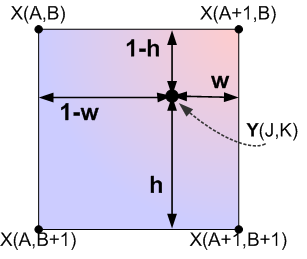
\includegraphics[scale=0.5]{../Figures/bilinear_interpolation.png}
			\caption{\label{fig:bilinear_img}Image from \url{https://www.giassa.net/?page_id=240}\cite{bilinear_img}}
		\end{figure}
		\begin{equation}
		\label{equ:bilinear}
		\centering
		Y(J,K)=(1-W)(1-H)X(A,B)+(W)(1-H)X(A+1,B)+(1-W)(H)X(A,B+1)+(W)(H)X(A+1,B+1)
		\end{equation}
	\subsection{Literature}
		\justifying Qingshuang et al.\cite{qingshuang2013parallel} proposed "GPGPU-based parallel algorithm can take full advantage of the GPU's parallel computing capabilities, and can achieve about 40 times speedup. (Table-\ref{tab:table_1})" \\
		\begin{table}[H] % H stands for here not anywhere else
			\centering	
			\caption[The Time-Consuming Of Serial And Parallel Bilinear Spatial Interpolation Of Different Grid Size]{\justifying The Time-Consuming Of Serial And Parallel Bilinear Spatial Interpolation Of Different Grid Size \cite{qingshuang2013parallel}}
			\label{tab:table_1}
			\begin{tabular}{l c c }
				Grid Size & CPU (sec) & GPU (sec)\\ \hline\hline 
				40x40 & 1.70 & 0.11 \\  \hline
				100x100 & 10.34 & 0.37 \\ \hline
				200x200 & 41.43 & 1.21 \\ \hline
				300x300 & 93.13 & 2.36 \\ \hline
				500x500 & 240.02 & 5.70 \\ \hline
				800x800 & 630.92 & 14.40 \\ \hline
				1200x1200 & 1432.33 &  32.41 \\ \hline
			\end{tabular}
		\end{table}
		
		\justifying Akgün and Gevrekci have been proposed "a massively multi-threaded implementation of super-resolution image formation on the NVIDIA CUDA architecture." \cite{akgun2013accelerating} "Super-resolution reconstruction begins with an initial estimate image which is typically chosen as a bilinearly upscaled version of the original low resolution frame." Their kernel's profile can be seen in Table-\ref{tab:table_2}.
		%table-2
		\begin{table}[H] % H stands for here not anywhere else
			\centering	
			\caption[Bilinear filtering code analysis]{Bilinear filtering code analysis \cite{akgun2013accelerating}}
			\label{tab:table_2}
			\begin{tabular}{l c}\hline\hline
				Thread numbers (x,y) &(32,32) \\ \hline 
				Shared memory bank conflict & N/A \\ \hline
				Global memory BW efficiency & 100 \\ \hline
				Register usage & 17 \\ \hline
				Occupancy & 0,877 \\ \hline
				Total execution time per frame & 161 microsec\\ \hline
			\end{tabular}
		\end{table}
	\subsection{Literature-Real Life Implementations}	
		\justifying There are multiple implementations using software /hardware acceleration on CPU/GPU. One of most used framework OpenCV has both CPU and GPU implementation of upsampling using bilinear interpolation.
		\vspace{1 cm}
		\begin{lstlisting}[language=C, caption={OpenCV Prototype of Bilinear Upsampling Function on CPU},label={lst:opencvcpu}]
void cv::resize (InputArray src, OutputArray dst, Size dsize, double fx=0, double fy=0, int interpolation=INTER_LINEAR		)
		\end{lstlisting} 
		\begin{lstlisting}[language=C,caption={OpenCV Prototype of Bilinear Upsampling Function on GPU}]
void cv::cuda::resize	(InputArray src, OutputArray dst, Size dsize, double fx = 0, double fy = 0, int interpolation = INTER_LINEAR, Stream &stream=Stream::Null())	
		\end{lstlisting}
		\vspace{1 cm}
		
		\justifying Intel offers developers high-quality, production-ready, low-level building blocks for image processing, signal processing, and data processing  applications by using a library called Intel® Integrated Performance Primitives (Intel® IPP). This library optimized for  wide range of Intel® architecture (Intel® Quark™, Intel Atom®, Intel® Core™, Intel® Xeon®, and Intel® Xeon Phi™ processors). Their bencmarks for image resizing is in Figure-\ref{fig:ipp_img_performance}. 

		\justifying Intel® IPP library unfortunately is not free. It's price starts from 249\$ for academic licence. OpenCV 3.x has native support for IPP-ICV library which is a special subset of Intel IPP functions for image processing and computer vision. 
		\vspace{1 cm}
		\begin{figure}[H]
				 	\centering
					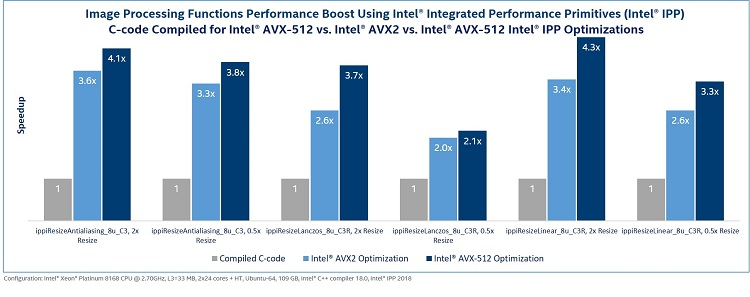
\includegraphics[scale=1.25]{../Figures/IPP2018-imageprocessing-performance.jpg}
					\caption{\label{fig:ipp_img_performance} Image from \url{https://software.intel.com}}
		\end{figure}
		\vspace{1 cm}
		\begin{lstlisting}[language=C,caption={Intel® IPP Prototype of Bilinear Upsampling Function}]
IppStatus ippiResizeLinear_<mod>(const Ipp<datatype>* pSrc, Ipp32s srcStep, Ipp<datatype>* pDst, Ipp32s dstStep, IppiPoint dstOffset, IppiSize dstSize, IppiBorderType border, const Ipp<datatype>* pBorderValue, const IppiResizeSpec_32f* pSpec, Ipp8u* pBuffer)
		\end{lstlisting}
		\vspace{1 cm}		
		
		\justifying ImageMagick is an another commonly used software, which can be instantiated over command line, has support for many media formats, and can be used for many operation over media files including image resizing. 
		\begin{lstlisting}[language=bash,caption={Sample code for image resizing.}]
$ convert input.jpg -scale 200% -interpolate bilinear output.jpg
		\end{lstlisting}

\bibliography{../References/ref.bib}
\bibliographystyle{ieeetr}
\end{document}          
